\chapter{Comparison with QUIJOTE-MFI Data}\label{ch:comparison_quijote}

In this chapter we compare values of atmospheric brightness temperature,
which we have obtained making use of the numerical methods described in
\autoref{ch:statistical_picture} and \autoref{ch:atm_variations}, with
measurements acquired by the QUIJOTE experiment.

In particular, we consider the values of $T_\text{atm}$ that have been measured by the
\emph{Multi-Frequency Instrument} (MFI). MFI is mounted on
the QT1 telescope, which is deployed at the Observatorio del Teide. It
operates since November 2012 in four bands centered at
\SIlist{11;13;17;19}{\giga\hertz}.

\section{QUIJOTE Data and Raw Simulations}

The QUIJOTE dataset is represented in \autoref{fig:quijote_dataset}.  It
includes measurements from a total of \num{444} MFI \emph{sky-dip}
observations, performed between December 2012 and February 2015. Sky-dip
observations are measurements of atmospheric emission performed scanning
the sky at variable elevations. On average, we have one observation every
\num{1.78} days. However, the time distribution of the data is quite
inhomogeneous. There are periods in which we have one observation every
sidereal day (sometimes two per day), but there are some extended periods
without observations.

\begin{figure}
        \centering
        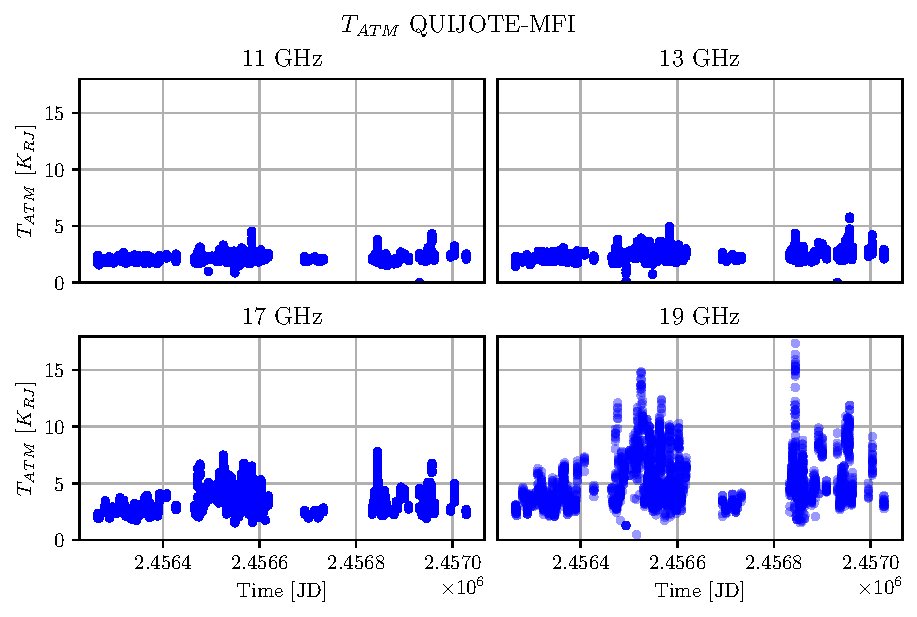
\includegraphics[width=\textwidth]{QUIJOTE_Dataset}
        \caption{QUIJOTE-MFI  $T_{atm}$ dataset.}
        \label{fig:quijote_dataset}
\end{figure}

For each point of the scatter plot showed in \autoref{fig:quijote_dataset},
we have used CAL to simulate a value of atmospheric brightness temperature
at the same frequency and at the same hour of a typical day of the
corresponding month. The comparison between simulated data and
$T_\text{atm}$ acquired by the QUIJOTE-MFI instrument is shown in
\autoref{fig:quijote_sim}.

\begin{figure}
        \centering
        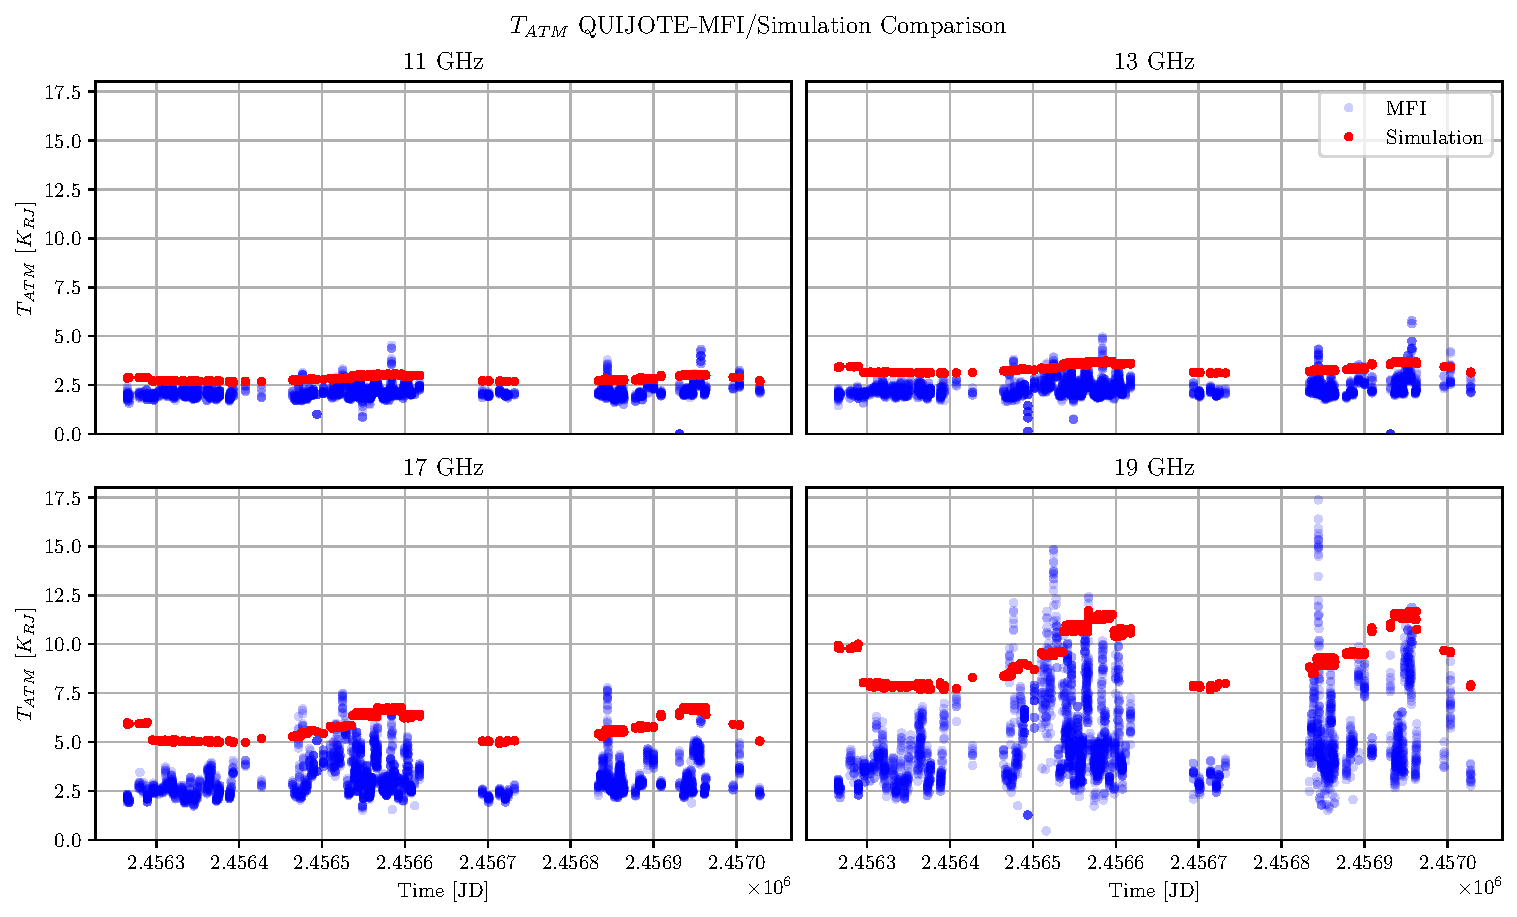
\includegraphics[width=\textwidth]{QUIJOTE-Sim}
        \caption{Comparison between QUIJOTE-MFI measurements and CAL
        simulated data.}
        \label{fig:quijote_sim}
\end{figure}

The scatter plot shows that a significant mismatch occurs. In particular
the simulations performed with CAL, making use of ERA5 dataset, yield
higher values of atmospheric brightness temperature. The mismatch is larger
at higher frequencies, approaching the \SI{22}{\giga\hertz} water vapour
line. Moreover, the QUIJOTE-MFI data exhibit larger fluctuations in time.

We recognise that part of the issues shown in \autoref{fig:quijote_sim}
are due to the insufficient spatial resolution of ERA5 reanalysis data.
\autoref{fig:pwv_teide_1980-01-01_12-00} shows a focus on the pixel in
which the Observatorio del Teide is located. In particular we are
interested in the area in which the Strip telescope will be deployed, which
in the figure is enclosed in a red circle. The ERA5 dataset only provides a
single value per hour of the PWV for the whole pixel, which constitutes a
spatial average.  Therefore, values of PWV are biased by contributions from
coastal low lands, below \SI{2390}{\meter}, and ocean waters. In other
words, the total column water vapour values that have been taken into
account to evaluate atmospheric brightness temperatures greatly exceeds
true values for Pico del Teide.

\begin{figure}
        \centering
        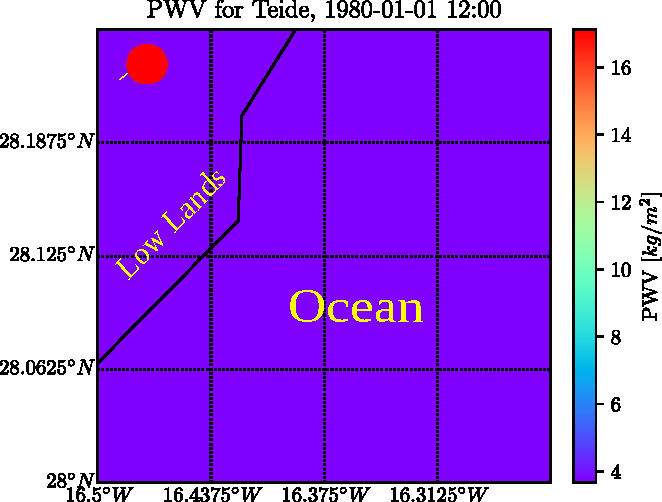
\includegraphics[width=0.80\textwidth]{PWV_Teide_1980-01-01_12-00}
        \caption{PWV for Pico del Teide.}
        \label{fig:pwv_teide_1980-01-01_12-00}
\end{figure}

\section{The Calibration Coefficient}

To mitigate part of the issues presented in the previous section, we have
used atmospheric vertical profiles of $T_s$, $P_s$ and PWV acquired by
balloon probes at Pico del Teide during 2018. These vertical
profiles reflect the true weather conditions near the observation site,
but are characterized by low temporal resolution. This is because balloon
probes need approximately \num{12} hours to measure a whole atmospheric
vertical profile. Therefore, no more than two vertical profiles per day can
be acquired.


The free and open source computer program \emph{Atmospheric Model}
(AM)\footnote{\url{https://zenodo.org/record/3406483}}
\autocite{paine2012atmospheric} has been used to compute sky brightness
temperatures starting from the  median annual vertical atmospheric profile
for the year 2018. AM is a tool for radiative transfer computations at
microwave to submillimeter wavelengths.  Spectra which can be computed with
AM include thermal emission, absorption, transmission, and excess delay.
Median annual values of $T_\text{sky}$ has been obtained in the frequency
range from \SIrange{10}{50}{\giga\hertz}, with a frequency step of
\SI{0.1}{\giga\hertz}.

To compare this result with sky brightness temperatures from CAL,
statistical populations of \num{2736000} elements for the relevant
meteorological parameters have been computed. As before, we have
initialized the \texttt{Weather} method with the CDFs \texttt{.fits} file
for Pico del Teide. The extracted values of PWV, $T_s$ and $P_s$, which are
shown in \autoref{fig:teide_annual_distributions}, are homogeneously
distributed among the months of the year and the hours of the day.
Expectation values for the meteorological parameters were computed from the
corresponding statistical populations using the same estimator choosen for
balloon vertical profiles. The annual median values and corresponding
standard errors for PWV, $T_s$ and $P_s$ are presented in
\autoref{tab:median_meteo_cal}.  These values have been used as input for
the \texttt{atm\_atmospheric\_loading} function to attain values of $T_\text{sky}$
in the appropriate frequency range.

\begin{figure}
        \centering
        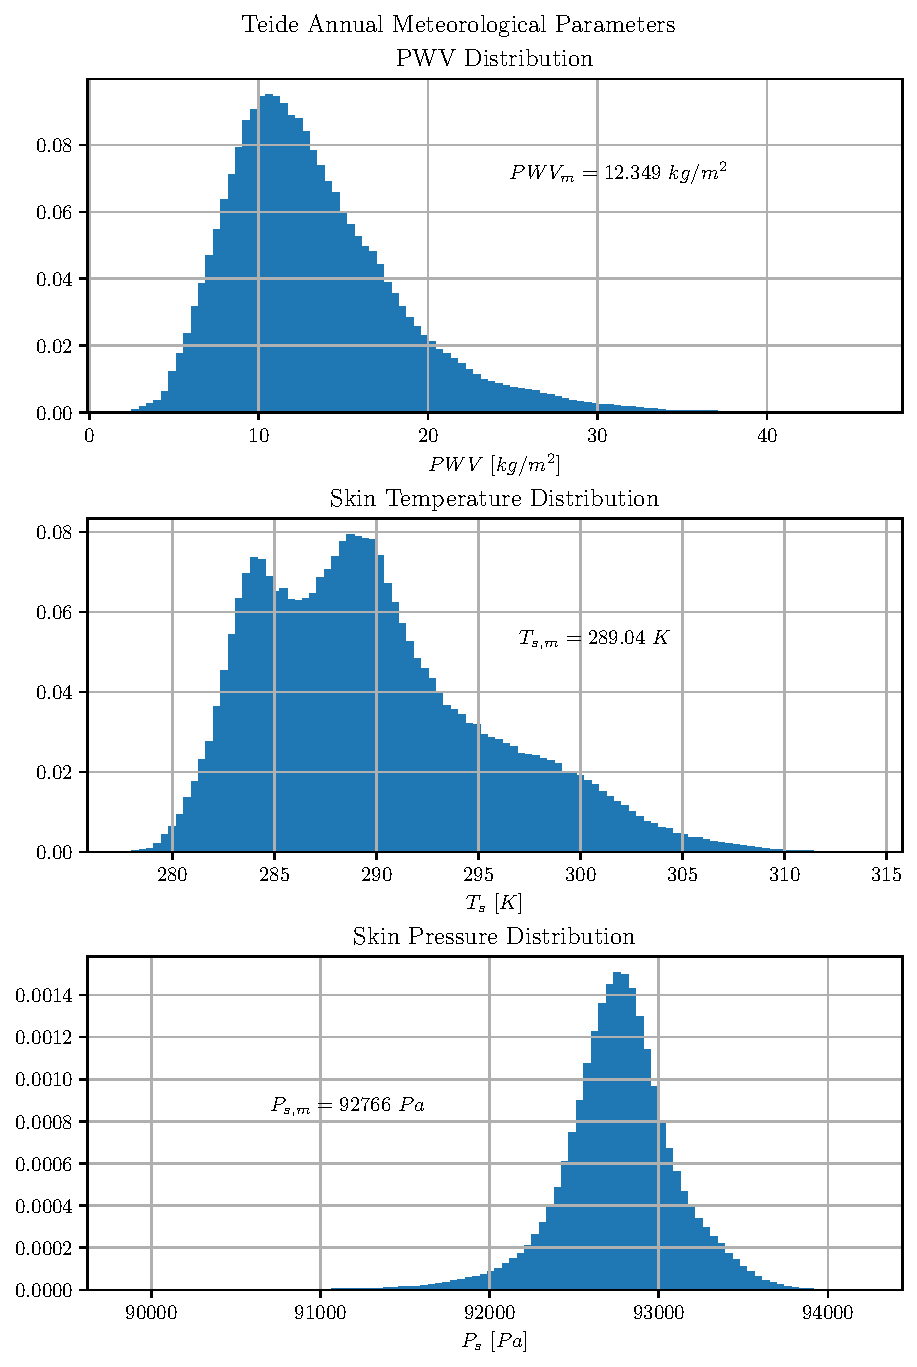
\includegraphics[width=0.93\textwidth]{Teide_Annual_Distributions}
        \caption{Annual distribution for relevant meteorological parameters
        at Pico del Teide obtained using CAL and ERA5 data.}
        \label{fig:teide_annual_distributions}
\end{figure}

\begin{table}
        \renewcommand{\arraystretch}{1.5}
        \centering
        \begin{tabular}{p{5cm} r}
                \hline
                Parameter & Median  \\
                \hline
                \hline
                PWV \dotfill & \SI{12.3491 \pm 0.0029}{\kilo\gram\per\square\meter} \\
                $T_s$ \dotfill& \SI{289.0434 \pm 0.0025}{\kelvin} \\
                $P_s$ \dotfill &  \SI{92766.55 \pm 0.21}{\pascal} \\
                \noalign{\smallskip}
                \hline
        \end{tabular}
        \caption{CAL median values of relevant meteorological parameters.}
        \label{tab:median_meteo_cal}
\end{table}

The sky brightness temperatures that have been computed making use of CAL
and AM are plotted as a function of $\nu$ in
\autoref{fig:am_cal_comparison}. As expected, the $T_\text{sky}$
from CAL assumes an higher value than that computed with the AM computer
program, when evaluated at the same
frequency. The distance between the two curves becomes particularly
significant near the \SI{22}{\giga\hertz} water vapour absorption line.

\begin{figure}
        \centering
        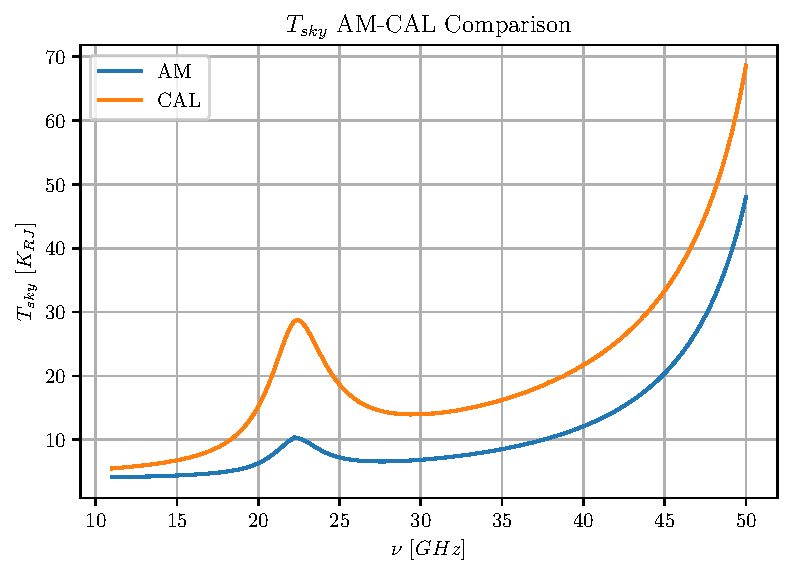
\includegraphics[width=\textwidth]{AM_CAL_Comparison}
        \caption{AM/CAL sky brightness temperatures comparison.}
        \label{fig:am_cal_comparison}
\end{figure}

We can now introduce a calibration coefficient, $k\qty(\nu)$, to correct
higher values in atmospheric brightness temperature computed by CAL, which
are caused by the excess in total column water vapour in ERA5 data for
the pixel in which the observation site is located. The coefficient is defined as

\begin{equation}
        k_\nu \equiv  k\qty(\nu) \equiv
        \frac{T^\text{AM}_\text{atm}\qty(\nu)}{
        T^\text{CAL}_\text{atm}\qty(\nu)}
\end{equation}

It must be noted that $k_\nu$ is assumed to be time independent. This means
that we think that weather conditions are homogeneous across the pixel, and
non-homogeneity in meteorological parameters at a fixed time only depends
on quantities which are not time dependent, such altitude and distance from
the ocean. This assumption could be veriefied acquiring multiple vertical
profiles simultaneously in the same pixel or performing radar scans of the
distribution of clouds and precipitations. The calibration coefficient as a
function of frequency is shown in
\autoref{fig:calibration_coefficient_quijote}.

\begin{figure}
        \centering
        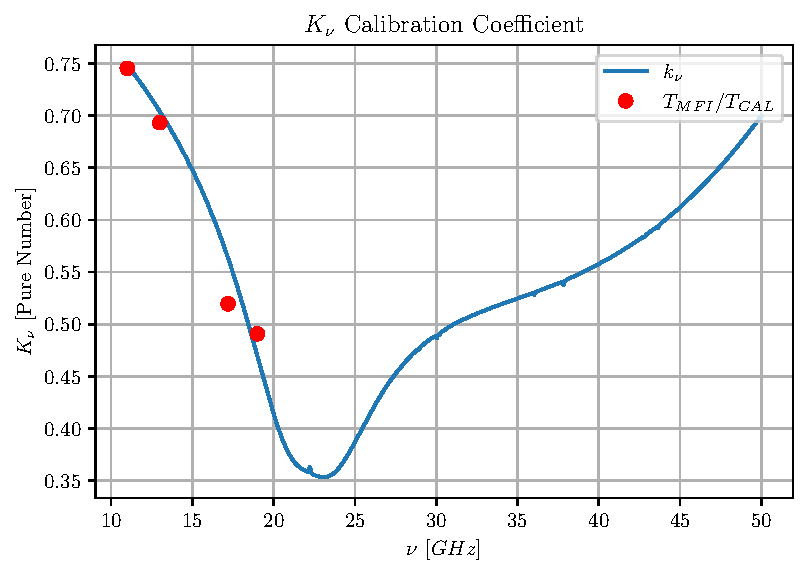
\includegraphics[width=\textwidth]{Calibration_Coefficient_QUIJOTE}
        \caption{$K_\nu$ calibration coefficient.}
        \label{fig:calibration_coefficient_quijote}
\end{figure}

The red dots in the figure represent the ratios between the median values of
atmospheric brightness temperatures measured by QUIJOTE-MFI and those of data
simulated with CAL. As it can be seen, they stand in proximity of the
blue line, confirming the validity of the calibration technique at least
for the MFI central frequencies.

\section{QUIJOTE Data and Calibrated Simulations}

The calibration coefficient defined in the previous section can be used to
correct \autoref{eq:tatm_formula}, which have been employed to calculate
atmospheric brightness temperatures with CAL:

\begin{equation}
        T_\text{atm}\qty(\nu) = k\qty(\nu)\qty[T_\text{sky}\qty(\nu) -
        T_\text{CMB}\qty(\nu)e^{-\tau_A\qty(\nu)}].
        \label{eq:tatm_formula_calibrated}
\end{equation}

\autoref{fig:quijote_sim_calibrated} shows the same comparison that has
been presented in \autoref{fig:quijote_sim}, but atmospheric brightness
temperatures obtained using \autoref{eq:tatm_formula_calibrated} are now
included. At a first glance, the calibrated simulations appear to be
compatible with QUIJOTE-MFI measurements.
\autoref{fig:quijote_sim_calibrated_residuals_boxplot} represents the
boxplot of the residuals for each frequency channel. The expectation values
of the distributions of residuals are compatible with zero for every
frequency within a \SI{95}{\percent} confidence level.

\begin{figure}
        \centering
        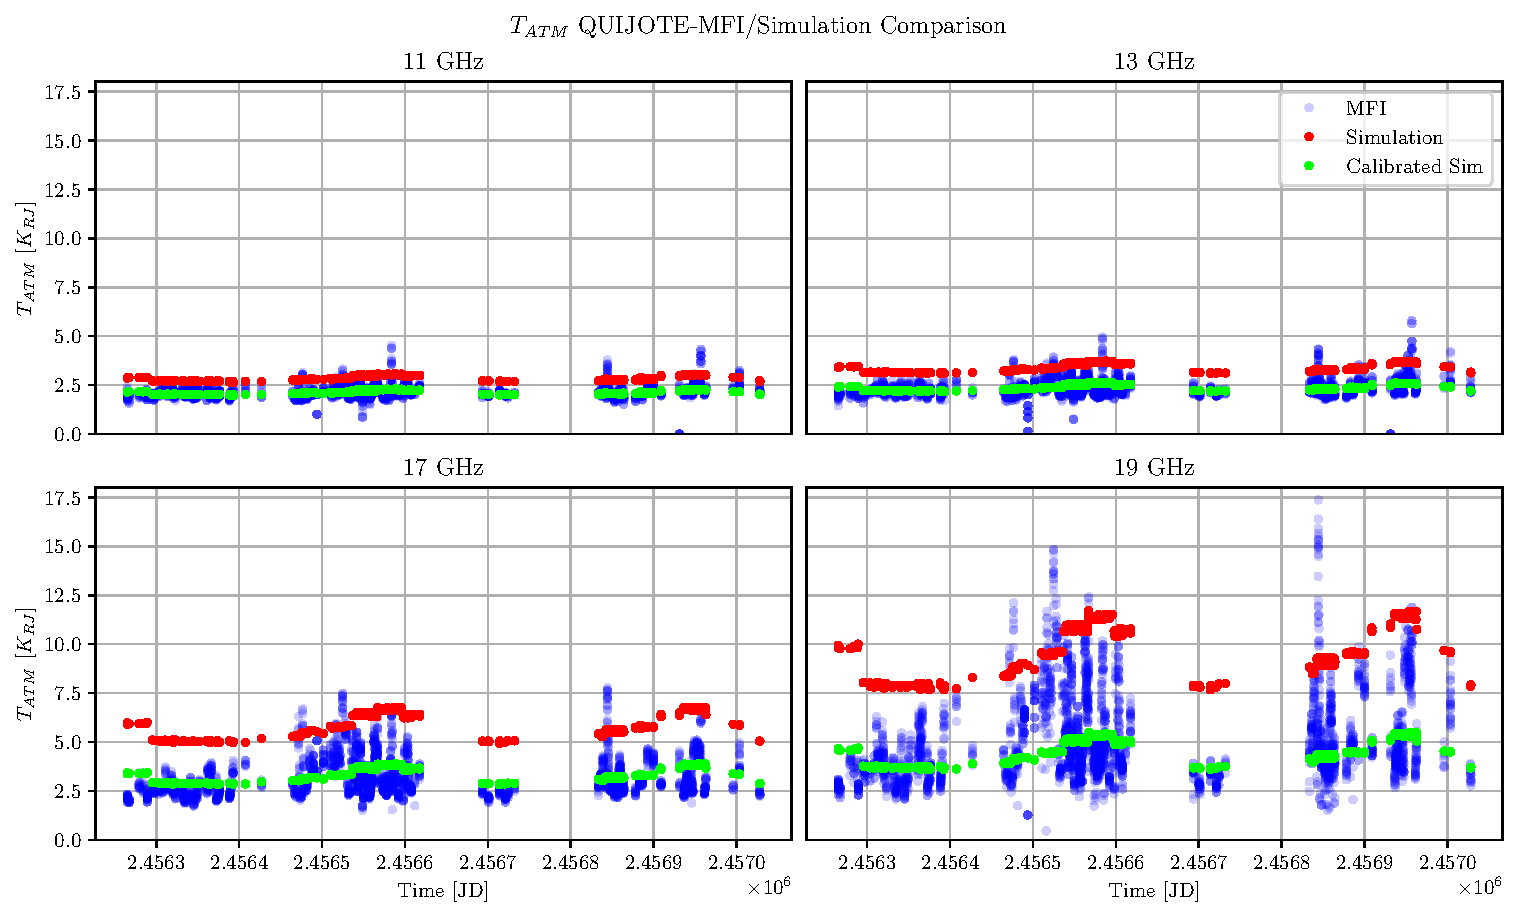
\includegraphics[width=\textwidth]{QUIJOTE-Sim_calibrated}
        \caption{Comparison between QUIJOTE-MFI measurements and
        CAL simulated data with calibration applied.}
        \label{fig:quijote_sim_calibrated}
\end{figure}

\begin{figure}
        \centering
        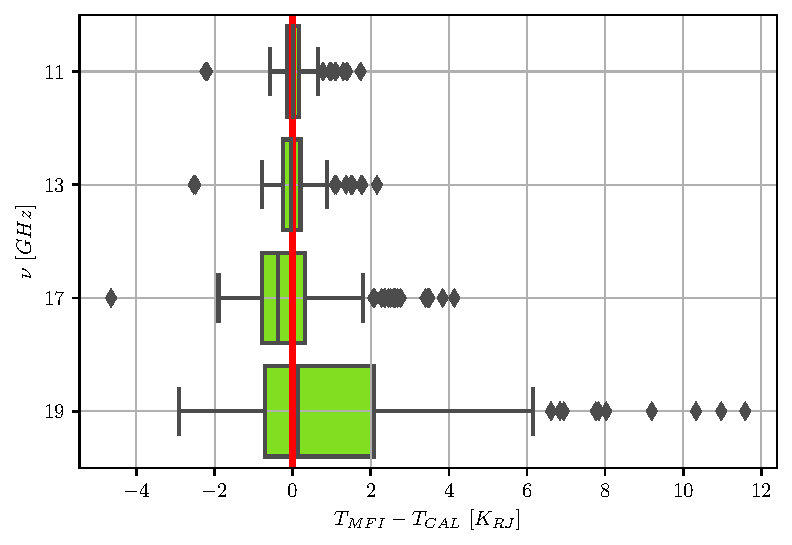
\includegraphics[width=0.93\textwidth]{QUIJOTE-Sim_calibrated_residuals_boxplot}
        \caption{Residuals for QUIJOTE-MFI measurements and
        CAL simulated data with calibration applied.}
        \label{fig:quijote_sim_calibrated_residuals_boxplot}
\end{figure}

However, our simulations can not reproduce fluctuations in atmospheric
brightness temperature and asymmetry in its distribution, which are
observed in particular for the \SI{19}{\giga\hertz} channel.  These
features appear to be more relevant for higher frequencies, approaching the
\SI{22}{\giga\hertz} water vapour absorption line. This suggests that the
dispersion in brightness temperature could be caused by the turbulent
structure of water vapour in the atmosphere, which has been discussed in
\autoref{ss:turbulent_structure}. It's easy to identify the white noise
contribution of the atmosphere at 19 GHz, but the presence of atmospheric
brightness fluctuations indicates that the atmosphere, at higher frequency,
is very complicated to model and the effects of the turbulent structures of
the water vapor are significant.  In conclusion, we can
estimate the average white noise contributions of the atmosphere but there
is another correlated contribute left to figure out.
